%%%%%%%%%%%%%%%%%%%%%%%%%%%%%%%%%%%%%%%%%%%%%%%%%%%
%
%  New template code for TAMU Theses and Dissertations starting Fall 2016.  
%
%
%  Author: Sean Zachary Roberson
%  Version 3.17.09
%  Last Updated: 9/21/2017
%
%%%%%%%%%%%%%%%%%%%%%%%%%%%%%%%%%%%%%%%%%%%%%%%%%%%
%%%%%%%%%%%%%%%%%%%%%%%%%%%%%%%%%%%%%%%%%%%%%%%%%%%%%%%%%%%%%%%%%%%%%%
%%                           SECTION IV
%%%%%%%%%%%%%%%%%%%%%%%%%%%%%%%%%%%%%%%%%%%%%%%%%%%%%%%%%%%%%%%%%%%%%



\chapter{EVENT RECONSTRUCTION \label{cha:eventreco}}
In the CMS detector, collisions happen in a small longitudinal region near the center called the luminous region or interaction region. Collisions themselves are not recorded, only the particles that get created. The origin of one or more new particles is called a vertex. An event is the set of particle measurements in the detector associated to a single beam-beam crossing. It is the job of the reconstruction software to process the raw information and identify physics objects for a given event.

 \begin{figure}[H]
 	\centering
 	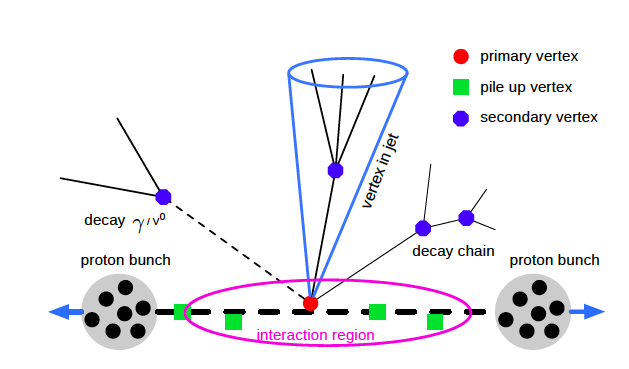
\includegraphics[width=0.75\textwidth]{figures/eventvertex.png}
 	\singlespace
 	\caption{Schematic diagram for an event at the LHC.}
 	\label{fig:vertex}
 \end{figure}


\section{Data Acquisition}
The CMS Data Acquisition (DAQ) and trigger system was specifically designed to collecte and analyze data at a rate of 40MHz, which corresponds to a 25 ns collision rate. Unfortunately, due the electronics system is only able to record a few hundreds of Hz of events. Therefore, events are filtered online by so-called trigger systems, so that only interesting events are written to disk. The collision triggering the readout is called the primary vertex, while other collisions from the beams are called pile-up. Secondary vertices refer to the other production points, when particles are created from decay or hard-scattering. This is shown in Figure \ref{fig:vertex}. Particles from the primary vertex usually have a high transverse momentum ($p_{T}$), making them interesting and easier to study.

\subsection{L1 Trigger and HLT}
 When CMS is performing at its peak, about one billion proton-proton interactions will take place every second inside the detector. In order to record only those events generated from energetic, head-on collisions, a "trigger" system was implemented.

Level 1 of the trigger is an extremely fast, hardware based process that looks for simple signs of interesting physics, e.g. particles with a large amount of energy or in unusual combinations. The L1 trigger selects events at a rate of around 100 kHz within a time interval of 4$\mu$s. The next step is the HLT, which combines the information from different parts of the detector to recreate the entire event and send it to a farm of more than 1000 computers to filter even more events, reducing the event rate to less than 1 kHz before recording them on tape.

\subsection{T1 sites and data storage}

CMS computing operates on a tiered computing structure. A Tier-0 computing center is located at CERN where the data is tranferred form the HLT and a first set of reconstruction occurs. From there, it is transferred to one of seven Tier-1 computing centers located around the world. At the Tier-1 centers, a full reconstruction of the data is performed. Furthermore, there are 55 Tier-2 centers which can be accessed by the collaboration members for data processing and storage.

 \begin{figure}[H]
 	\centering
 	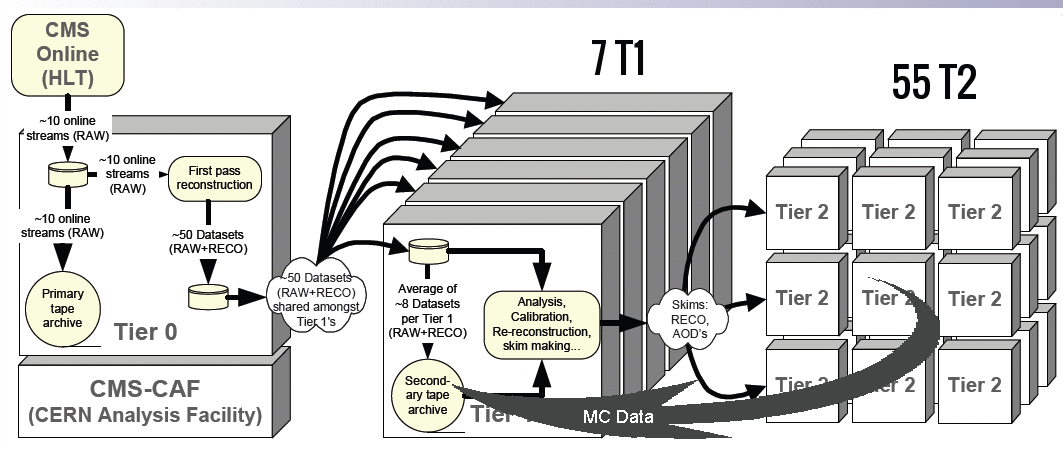
\includegraphics[width=0.75\textwidth]{figures/dataflowtiers_MC.gif}
 	\singlespace
 	\caption{Flow of CMS detector data through the tiers. Reprinted from \cite{CMSdatatier}}
 	\label{fig:datatier}
 \end{figure}

 The data itself is also processed in three data tiers. The first layer of this is the RAW data, which is created by unpacking detector streams passed on from the L1 and HLT triggers, typically composed of measurements from the different calorimeters as well as some information provided by the L1 trigger. This RAW data is reconstructed into physics objects(i.e. muons, electrons, photons) that can be grouped later for further analysis. This step is called RECO, which is short for reconstruction and contains both the detector and physics object information. 

 After RECO, an \textit{analysis object data} (AOD) is formed from a subset of the RECO information. AOD objects are typically comprised of only high-level physics objects, making the files much smaller. This data format is usually the preferred one for physics analysis.



\section{Particle Flow Event Reconstruction}
\label{sec:track}

As mentioned in Section 2, CMS is one of the two general-purpose detectors at the LHC, and as such, it was designed based on the concept of cylindrical detection layers. In the previous section we described how data was managed and stored during the acquisition process. This section will focus on how physicists make sense of the raw detector information.  

 First, detector data is measured in the form of electronig signals, i.e. hits in the tracker or energy depositions in the calorimeters. Then, the trajectories of charged particles, or tracks, are reconstructed from the position hits in the detector. From the collection of tracks in an event, the primary and any secondary vertices are reconstructed. 

An optimal event description can be achieved by correlating the basic elements from all detector layers (tracks and clusters) to identify each final-state particle, and by combining the corresponding measurements to reconstruct the particle properties on the basis of this identification. At CMS, this approached is called \textit{particle-flow (PF) reconstruction}.

The reconstructed and identified individual particle list includes muons, electrons, photons, charged hadrons, as well as stable and unstable neutral hadrons. These particles can be non-isolated, and even originate from an intricate overlap of reconstructed charged particles, ECAL and HCAL energy clusters, and signals in the muon chambers.

Looking at Figure \ref{fig:cmsslice}, one can see that photons and neutral hadrons are in general identified by ECAL and HCAL clusters with no track link. No attempt is made to distinguish the various species of neutral and charged hadrons in the PF reconstruction. Electrons can be identified by a track and an ECAL cluster, with a momentum-to-energy ratio compatible with unity, and not connected to an HCAL cluster. Finally, muons and neutrinos would traverse the calorimeters with little or no interactions. While neutrinos would escape undetected, muons would be identified by a track in the inner tracker connected to a track in the muon detectors.

 \begin{figure}[h]
  	\label{fig:cmsslice}
 	\centering
 	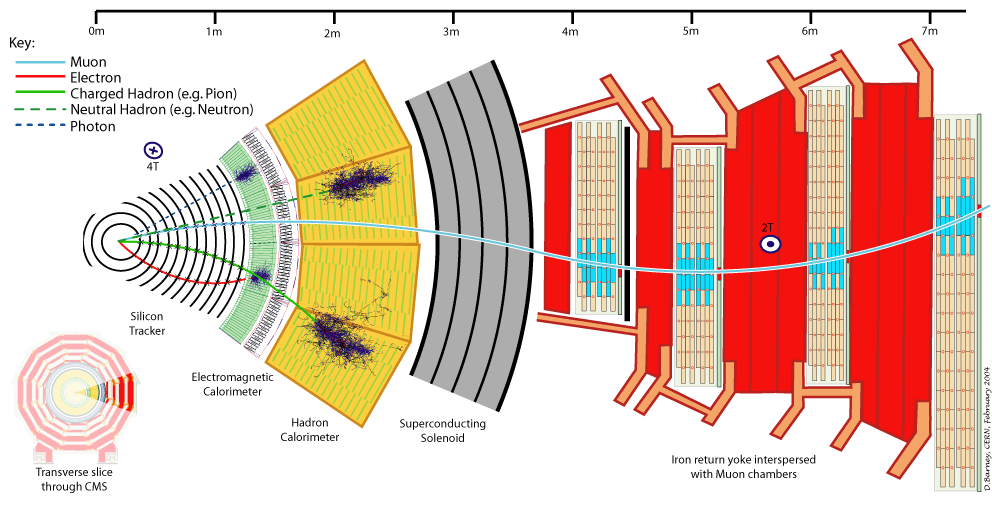
\includegraphics[width=0.75\textwidth]{figures/image005.gif}
 	\singlespace
 	\caption{Cross-sectional view of the CMS detector with all of the sub-detectors labeled. The colored lines correspond to different particle types. Each particle interacts with different pieces of the detector and may or may not be bent by the magnetic field. Reprinted from \cite{CMSSlice}}
 \end{figure}

The PF concept was developed and used for the first time by the ALEPH experiment at LEP\cite{BUSKULIC1995481} and can now be used in hadron colliders due to the very fine spatial granularity of the detectors. In particular, CMS is very well suited for PF reconstruction due to its highly-segmented tracker,  a fine-grained ECAL, and an hermetic HCAL.

Also, the CMS magnet is large enough to accomodate the tracker and both the ECAL and HCAL, thereby minimizing the mount of material in front of the calorimetes. This particular feature is an advantage for PF reconstruction, as it eliminates the energy losses before the calorimeters caused by particles showering in the coil material and facilitates the link between tracks and calorimeter clusters.

\subsection{Iterative Tracking}

 The first step of the reconstruction process is referred to as local reconstruction and it consists of the clustering of \textit{zero-suppressed} signals above specified thresholds in pixel and strip channels into hits. The next step is track reconstruction, which refers to the process of using the reconstructed hits to obtain estimates for the momentum and position parameters of the charged particles responsible for the detector hits. 

 The tracking software at CMS\cite{TRK-11-001} is commonly referred to as the combinatorial Track Finder (CTF), which is an adaptation of the combinatorial Kalman Filter \cite{Billoir:1989mh},\cite{BILLOIR1990219},\cite{Mankel:1997dy}, which in turn is an extension of the Kalman filter\cite{Fruhwirth:1987fm} to allow pattern recognition and track fitting to occur in the same framework. The collection of reconstructed tracks is produced by multiple passes or iterations of the same CTF track reconstruction sequence, in a process called iterative tracking. 

The basic idea of iterative tracking is that the initial iteration seach for tracks that are easiest to find (e.g., of relatively large $p_{T}$, and produced near the interaction region). After each iteration, hits associated with tracks are removed, thereby reducing the combinatorial complexity, and simplifying subsequent iterations in a seach for more difficult classes of tracks (e.g., low $p_{T}$, or greatly displaced tracks).

Each iteration proceeds in four steps:

\begin{itemize}
	\item Seed generation which provides track candidates consisting of a few (2 or 3) hits. Seeds are generated in the innermost layers of the tracker and are commonly reffered to as "proto-tracks".
	\item Track finding, which is based on a Kalman filter. It extrapolates the seed trajectories along the expected flight path of a charged particle, searching for additional hits that can be assigned to the track candidate.
	\item Track fitting. A module that is used to provide the best possible estimate of the parameters of each trajectory by means of a Kalman filter.
	\item Track selection. This step sets the quality flags and discards tracks that fails certain specified criteria.
\end{itemize}

A total of six iterations are used, each with different seed generation, $p_{T}$ and impact parameter requirements.

The first iterations have strict criteria in order to achieve a negligible small fake rate. Once the hits are associated with these tracks are removed, the seeding criteria is loosened. By doing this, tracking efficiency is increased. From iteration 4 and on, the constraints on the tracks closer to the interaction point are slowly relaxed. This allows for reconstruction of secondary charged particles created from photon conversions and nuclear interactions in the tracker volume.

\subsection{Calorimeter Clustering}
Clustering in the calorimeters is the process of grouping detector cells that register hits together to measure the energy and direction of stable neutral particles. Additionally, clustering seeks to separate the neutral particles from energy deposits associated with charged hadrons, reconstruct electrons (including all associated Bremsstrahlung photons), and measure the energy of charged hadrons for which tracks were not determined accurately. The clustering algorithm is performed separately in each subdetector: ECAL barrel and endcap, HCAL barrel and endcap, and in the preshower.

The clustering proceeds via three steps\cite{CMS:2009nxa}:

\begin{enumerate}
	\item Identify 'cluster seeds'. These are defined as the cell in a calorimeter with a local maximum of energy (above some set threshold).
	\item Expand from the seed to grow 'topological clusters'. This is done by aggregating calorimeter cells that have at least one side in common with the seed cell, and also have an energy over a particular threshold.
	\item Repreat the process of cluster growing, now using new cells that are part of the cluster.
\end{enumerate}

In this sense, a "seed" gives rise to a "particle-flow cluster". If a cell is identified by two clusters, the energy is shared between the clusters according to the distance from the cell to the center of each cluster. The cluster energies and positions are iteratively determined as new cells are added to the cluster.

\subsection{Linking Tracks and Clusters}
Once the basic PF elements like the trajectories of charged particles in the inner tracker, electron and muon tracks, and calorimeter clusters are available, the next step in reconstructing a particle is the so-called \textit{link algorithm}.

 The link algorithm can test any pair of elements in the event. In order to prevent the computing time of the link algorithm from growing quadratically with the number of particles, the pairs of elements considered by the link procedure are restricted to the nearest neighbours in the ($\eta,\phi$) plane, as obtained with a $k$-dimensional tree\cite{Bentley1975MultidimensionalBS}. The specific conditions reuired to link two elements depend on their nature.

 If two elements are found to be linked, the algorithm defines a distance between these two elements, aimed at quantifying the quality of the link. The link algorithm then produces \textit{PF blocks} of elements associated either by a direct link or by an indirect link through common elements.

 The link between tracks and calorimeter clusters proceeds by extrapolating the last measured hit in the tracker to one of the three detectors\cite{CMS:2009nxa}:

 \begin{itemize}
 	\item The two layers of the preshower detector,
 	\item the ECAL, at a depth corresponding to the expected maximum of the electron shower profile,
 	\item the HCAL, to a depth corresponding to one interaction length.
 \end{itemize}

 The track is then linked to a cluster in these detectors if the extrapolated position is within the cluster boundaries. Additionally, to link Bremsstrahlung photons to their associated electron, tangents to the track are extrapolated to the ECAL and cluster found within those boundaries is also linked.

 Similarly, links between the calorimeters are formed when a cluster from the more granular calorimeter (preshower or ECAL) is within the cluster envelope os the less granular calorimeter (ECAL or HCAL).

 Finally, muon tracks are linked to charged particle tracks by a global fit between the two sets of tracks.

 \section{Physics Object Reconstruction}

With the tracks identified, calorimeter clusters formed and the linking of clusters to tracks, particles can then be reconstructed. The particle flow process begins by reconstructing muons, then electrons and photons, and finally charged hadrons. As each particle is reconstructed, the tracks and clusters associated with it are removed from the collection of blocks used to form candidate particles, which ensures that energy deposits attributed to one particle are not used twice. The hadrons are then clustered together to form jets, and these jets can additionally be identified as coming from tau leptons or b quarks (Figure \ref{fig:pf}).


 \begin{figure}[h]
  	\label{fig:pf}
 	\centering
 	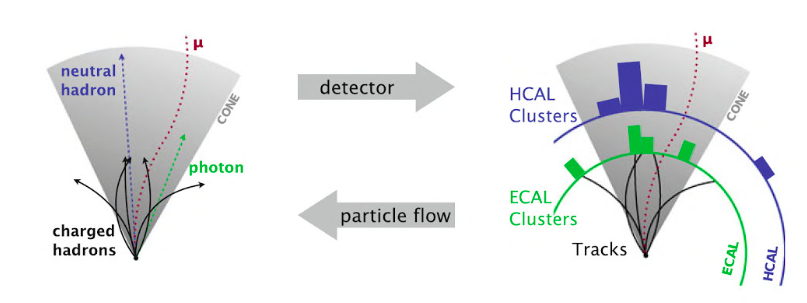
\includegraphics[width=0.75\textwidth]{figures/jets.png}
 	\singlespace
 	\caption{CMS Particle Flow algorithm. The diagram shows how collisions lead to particle decays and final state particles. On the right side of the diagram the tracks and deposits in the CMS detector are shown. The left side shows that PF candidates are derived from detector information and then become inpur for the PF algorithm that uses them to construct high-level physics objects like electrons, which are then used by analysts to reconstruct the collision event. Reprinted from \cite{CMS-PAS-PFT-09-001}}
 \end{figure}

\section{Jets}

During proton-proton collisions, the confined state of quarks and gluons is broken. This de-confined state of the free partons does not last very long, as it is not allowed by QCD. Shortly after the collision, partons hadronize and a bunch of particles is generated by this process. These particles are usually collimated in a given direction due to the boosted nature of the parton, and thereby producing a jet or spray of particles around it.

In practice, jets are the result of clustering groups of charged hadrons, photons, and neutral hadrons coming from PF. The energy fraction in jets is divided amongst them with a breakdown of roughly 65$\%$, 25$\%$, and 10$\%$ respectively. This is illustrated in Figure. For this study, jets were reconstructed from PF candidates clusters using the anti-$k_{T}$ algorithm\cite{Cacciari:2008gp} as defined in the FASTJET package\cite{Cacciari:2011ma}.

 \begin{figure}[h]
  	\label{fig:antikt}
 	\centering
 	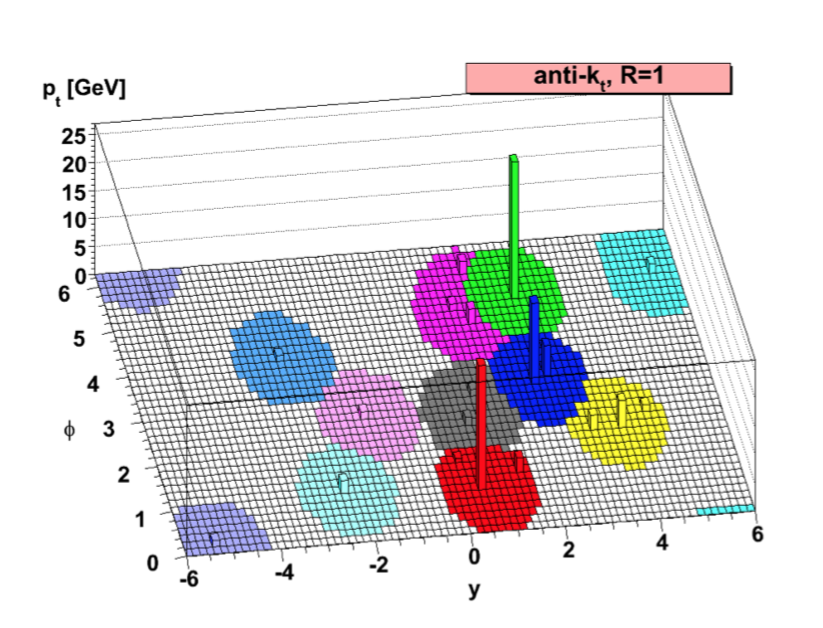
\includegraphics[width=0.75\textwidth]{figures/antikt.png}
 	\singlespace
 	\caption{A sample parton-level event clustered with the anti-$k_{T}$ algorithm. Reprinted from \cite{Cacciari:2008gp}}
 \end{figure}

 Jet clustering algorothms work by defining a distance parameter($d_{ij}$) between to PF candidates $i$ and $j$, and the distance between such cluster and the beam, $d_{iB}$. These are defined as

 \begin{align}
 \label{jetclust}
 d_{ij} = min(k_{ti}^{2p},k_{tj}^{2p})\frac{\Delta_{ij}^{2}}{R^{2}}
 d_{iB} &= k_{ti}^{2p}
 \end{align}

where $\Delta_{ij}^{2} = (y_{i}-y_{j})^{2}+(\phi_{i}-\phi_{j})^{2}$, and $k_{ti}$, $y_{i}$, and $\phi_{i}$ are the transverse momentum, rapidity, and azimuth of particle $i$, respectively. R is a user-defined radius parameter, and $p$ is a measure of the relative power of energy vs geometric scales. Particularly, for the anti-$k_{T}$ algorithm, $p=-1$, and Equation \ref{jetclust} reduces to

\begin{equation}
 d_{ij} = min(\frac{1}{p_{ti}^{2}},\frac{1}{p_{tj}^{2})\frac{\Delta_{ij}^{2}}{R^{2}}
\end{equation}

The algorithm loops over all PF candidate objects, calculating $d_{ij}$ for each pair of objects. Once it does this, it selects the two objects with the lowest value of $d_{ij}$ and combines them. This process is repeated until the smallest value of $d_{ij}>d_{iB}$ for all the remaining pairs. 

As a result, the cutoff limit of $1/p_{T}^{2}$ defines a maximum size that the algorithm will look to cluster particles inside. The construction of $d_{ij}$ using the inverse $p_{T}^{2}$ has a result of producing values of $d_{ij}$ that are smaller for objects with a higher $p_{T}$, given equal separation. As a result, softer particles will tend to cluster to higher $p_{T}$ particles long before they would cluster amongst themselves. If no hard particles are present, the jet object will simply cluster soft $p_{T}$ particles in a circle in an $\eta-\phi$ space of radius R.

The clustering of the anti-$k_{T}$ algorithm leads to jets with a large $p_{T}$ being reconstructed as perfect circles, while softer jets can have a more ambiguous shape. Figure \ref{fig:antikt} shows a display of the anti-$k_{T}$ algorithm for a distance parameter R=1. Notice that the green jet around $y=2$ and $\phi=5$ has a circular shape, while it deforms the smaller jet right next to it.


\section{b-tagging}

\section{Event Generation}

\section{Detector Simulation}

